\documentclass[conference]{IEEEtran}

\usepackage[utf8]{inputenc}
\usepackage[T1]{fontenc}
\usepackage{graphicx}
\usepackage{float}
\usepackage{amsmath}
\usepackage{hyperref}
\usepackage{xcolor}
\usepackage{booktabs}
\usepackage{caption}
\hypersetup{colorlinks=true, linkcolor=blue, urlcolor=blue, citecolor=blue}

% ─────────────────────────────────────────────────────────────────────────────
\begin{document}

\title{NBA Statistics Dashboard:\\
Visualizing 80 Years of Basketball Evolution}

\author{%
  \IEEEauthorblockN{Nurettin Macit}
  \IEEEauthorblockA{Istanbul Technical University\\macit22@itu.edu.tr}
  \and
  \IEEEauthorblockN{Mehmet Arda Öncel}
  \IEEEauthorblockA{Istanbul Technical University\\oncel23@itu.edu.tr}
  \and
  \IEEEauthorblockN{Yusuf O\u{g}uz}
  \IEEEauthorblockA{Istanbul Technical University\\oguz22@itu.edu.tr}
}

\maketitle

% ── Abstract ──────────────────────────────────────────────────────────────────
\begin{abstract}
This paper presents an interactive data visualization dashboard built on 80 years of NBA statistics (1947--2024). Using a Streamlit application with five thematic tabs, we explore five research questions: the transformation of gameplay driven by the three-point shot, relationships between physical attributes and performance, career arc and peak age patterns, the geographic origin of players, and statistical differences across playing positions. Visualizations are implemented in Plotly and cover time series, scatter plots, choropleth maps, heatmaps, and radar charts.
\end{abstract}

\begin{IEEEkeywords}
data visualization, NBA, basketball analytics, Streamlit, Plotly, sports analytics
\end{IEEEkeywords}

% ── I. Introduction ───────────────────────────────────────────────────────────
\section{Introduction}

The NBA is one of the most data-rich professional sports leagues in the world. Since its founding in 1946, the league has undergone fundamental tactical, physical, and demographic transformations. This work presents an interactive dashboard that visualizes nearly 80 years of basketball data, addressing five research questions (RQs):

\begin{itemize}
  \item \textbf{RQ1:} How has the three-point shot transformed gameplay?
  \item \textbf{RQ2:} Is there a relationship between physical attributes and performance?
  \item \textbf{RQ3:} How does performance develop across a career?
  \item \textbf{RQ4:} Which countries and U.S. states produce the most players?
  \item \textbf{RQ5:} How do statistical profiles differ across positions?
\end{itemize}

% ── II. Dataset ───────────────────────────────────────────────────────────────
\section{Dataset}

\subsection{Main Dataset}
The primary dataset is \textit{NBA Players \& Teams Statistics (1947--2024)} compiled from Basketball Reference and published on Kaggle~\cite{main_dataset}. It consists of 22 CSV files covering per-game player statistics, advanced metrics, team summaries, and draft history (33,278 rows, 11~MB). Key files used are \texttt{Player Per Game}, \texttt{Team Stats Per Game}, \texttt{Team Summaries}, and \texttt{Advanced}.

\subsection{Supplementary Datasets}
Two additional datasets are merged to fill gaps in the main source. \textit{NBA Players Data}~\cite{justinas_dataset} (12,844 rows, 1996--2023) provides \texttt{country}, \texttt{player\_height} (cm), and \texttt{player\_weight} (kg) used for RQ2 and RQ4. \textit{NBA Players by State}~\cite{birthplace_dataset} (3,407 rows, all-time) provides \texttt{City} and \texttt{State} birth information for the U.S. choropleth in RQ4.

\subsection{Preprocessing}
All analyses filter to regular season data only. Supplementary datasets are joined to the main dataset via lowercase player-name normalization. The birthplace file contained 280 columns due to a wide-format scraping artifact; only 14 relevant columns were retained. A minimum threshold of 20 games per season is applied for career arc analysis (RQ3) to exclude injury-shortened appearances. Season labels of the form \texttt{'1996-97'} are converted to end-year integers for cross-file joins.

% ── III. Visualizations ───────────────────────────────────────────────────────
\section{Visualizations}

\subsection{RQ1 -- Three-Point Revolution}

Team-level data from \texttt{Team Stats Per Game} is aggregated by season to compute the league-wide mean 3-point attempts (3PA) per game. Using team-level rather than player-level averages is essential: a per-player average yields $\approx3$ 3PA/game and obscures the trend, while the team-level value correctly reflects the 3.1 $\to$ 35.6 growth between 1980 and 2024.

Three charts are provided: (1) an area chart of team 3PA per game annotated with the 1979--80 rule introduction and the 2015--16 inflection point, (2) a dual-axis line chart comparing team scoring and pace, and (3) a bar chart of 3PA as a share of all field goal attempts.

\begin{figure}[H]
  \centering
  % ── HOW TO GET THIS FIGURE ──────────────────────────────────────────────
  % Open app: streamlit run app.py
  % Navigate to Tab 1 "Three-Point Revolution"
  % Set slider to 1979–2024
  % Take a screenshot showing the area chart (3PA/game)
  % Save as fig1.png in the same folder as this .tex file
  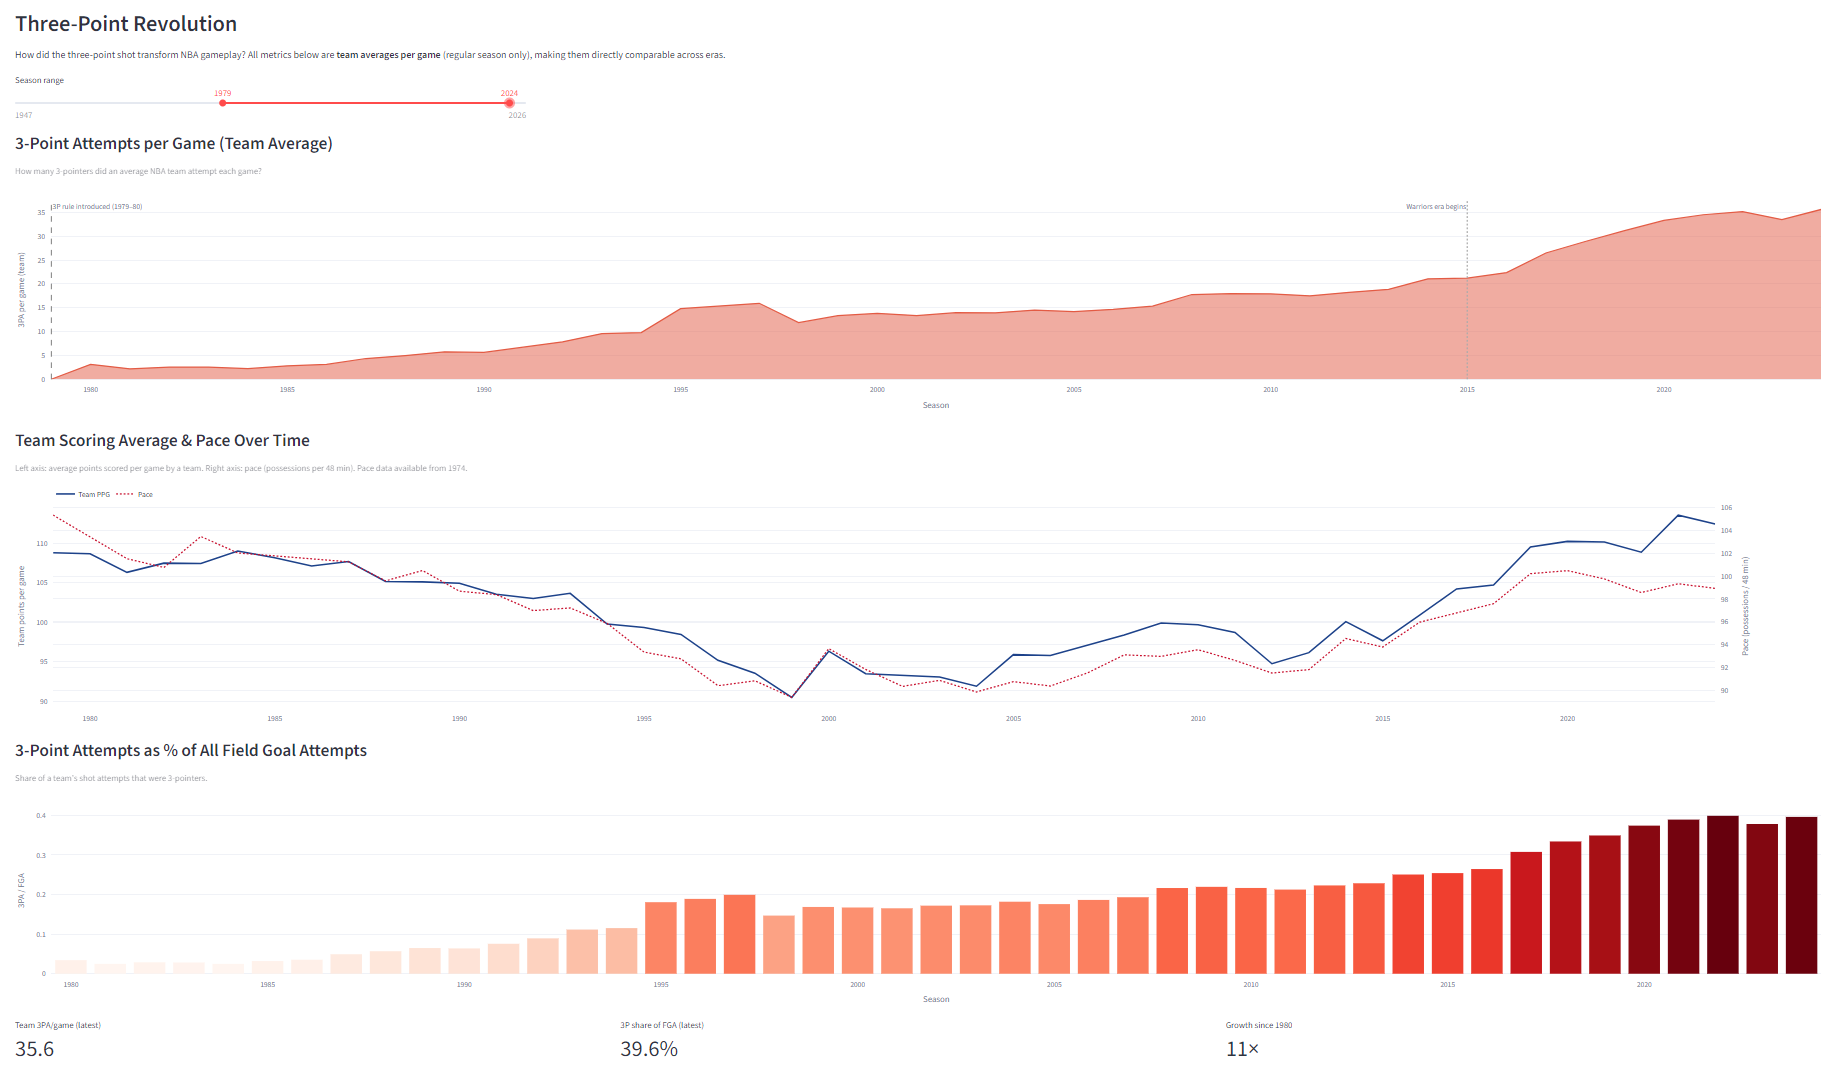
\includegraphics[width=\columnwidth]{figures/report/fig1.png}
  \caption{League-wide team 3-point attempts per game (1979--2024). The dashed line marks the 1979--80 rule introduction; the dotted line marks the 2015--16 Warriors era.}
  \label{fig:threept}
\end{figure}

Key finding: the 3PA share of all FGA grew from 3.4\% (1980) to 39.6\% (2024), representing an 11$\times$ increase in absolute attempts.

\subsection{RQ2 -- Physical Attributes vs Performance}

Height and weight from the supplementary dataset are joined with Win Shares and BPM from \texttt{Advanced}. A scatter plot with an OLS trendline (computed via \texttt{statsmodels}) is shown for user-selected axis combinations; a box plot displays physical attribute distributions across scoring quartiles.

\begin{figure}[H]
  \centering
  % ── HOW TO GET THIS FIGURE ──────────────────────────────────────────────
  % Navigate to Tab 2 "Physical vs Performance"
  % Set X: Height (cm), Y: Points per game
  % Take a screenshot showing the scatter plot with the red OLS trendline
  % Save as fig2.png
  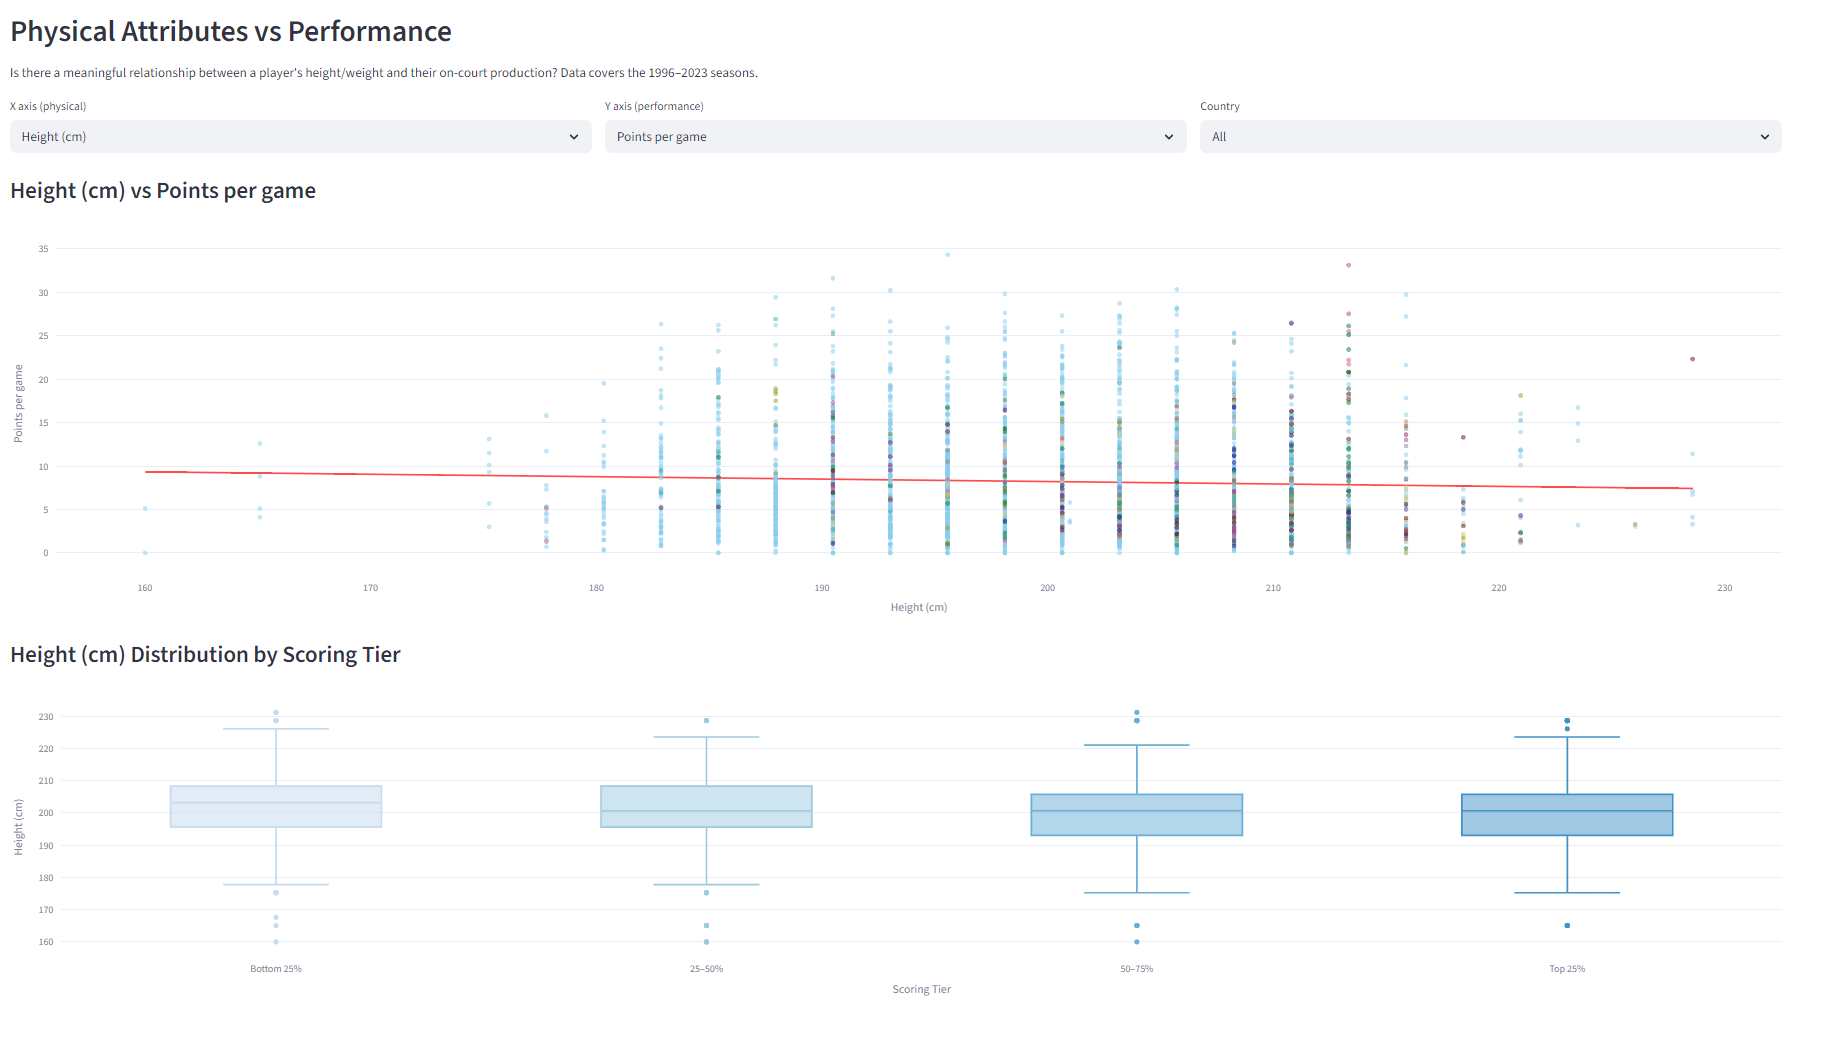
\includegraphics[width=\columnwidth]{figures/report/fig2.png}
  \caption{Height (cm) vs Points per game (1996--2023). Red line: OLS trendline. Each point is one player-season, colored by country of origin.}
  \label{fig:physical}
\end{figure}

Key finding: height shows a weak negative correlation with scoring (taller players accumulate value through rebounds and defense rather than volume scoring), while weight shows minimal correlation with any offensive metric.

\subsection{RQ3 -- Career Arc and Peak Age}

Per-game statistics from \texttt{Player Per Game} are grouped by age (18--40, min.\ 20 games/season) to produce league-wide average curves. A multi-line chart, a normalized heatmap, and a bar chart of player-season counts by age are provided.

\begin{figure}[H]
  \centering
  % ── HOW TO GET THIS FIGURE ──────────────────────────────────────────────
  % Navigate to Tab 3 "Career Arc & Peak Age"
  % Select all 3 stats (Points, Assists, Rebounds)
  % Take a screenshot of the multi-line chart + the blue peak-age info box
  % Save as fig3.png
  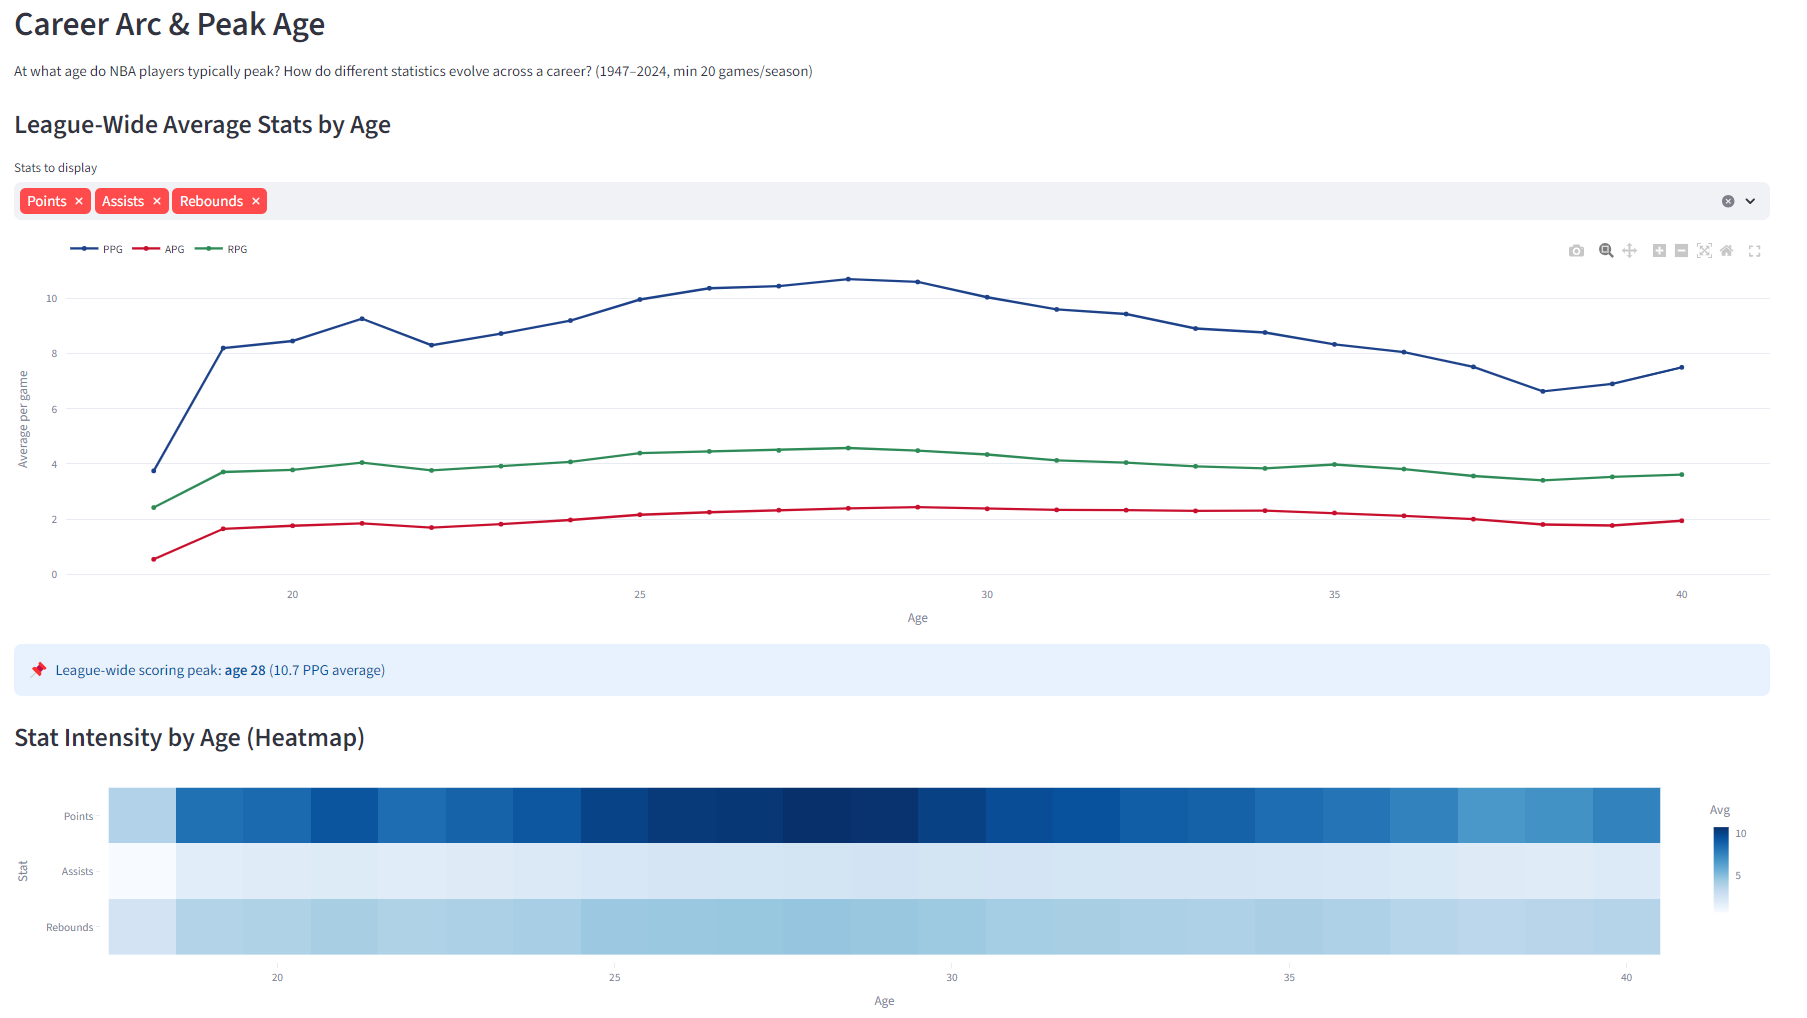
\includegraphics[width=\columnwidth]{figures/report/fig3.png}
  \caption{League-wide average PPG, APG, and RPG by player age (1947--2024, min.\ 20 games/season).}
  \label{fig:career}
\end{figure}

Key finding: scoring peaks at age 26--27; assists peak slightly earlier at 24--25. The sample thins sharply after 35, reflecting survivorship bias.

\subsection{RQ4 -- Geography}

The supplementary country dataset is aggregated by \texttt{country} to produce a world choropleth; the birthplace dataset is aggregated by \texttt{State} to produce a U.S. choropleth. Both maps support color encoding by player count or average statistics.

\begin{figure}[H]
  \centering
  % ── HOW TO GET THIS FIGURE ──────────────────────────────────────────────
  % Navigate to Tab 4 "Geography"
  % Set color-by to "# of Players"
  % Take a screenshot of the world choropleth (top of tab)
  % Save as fig4.png
  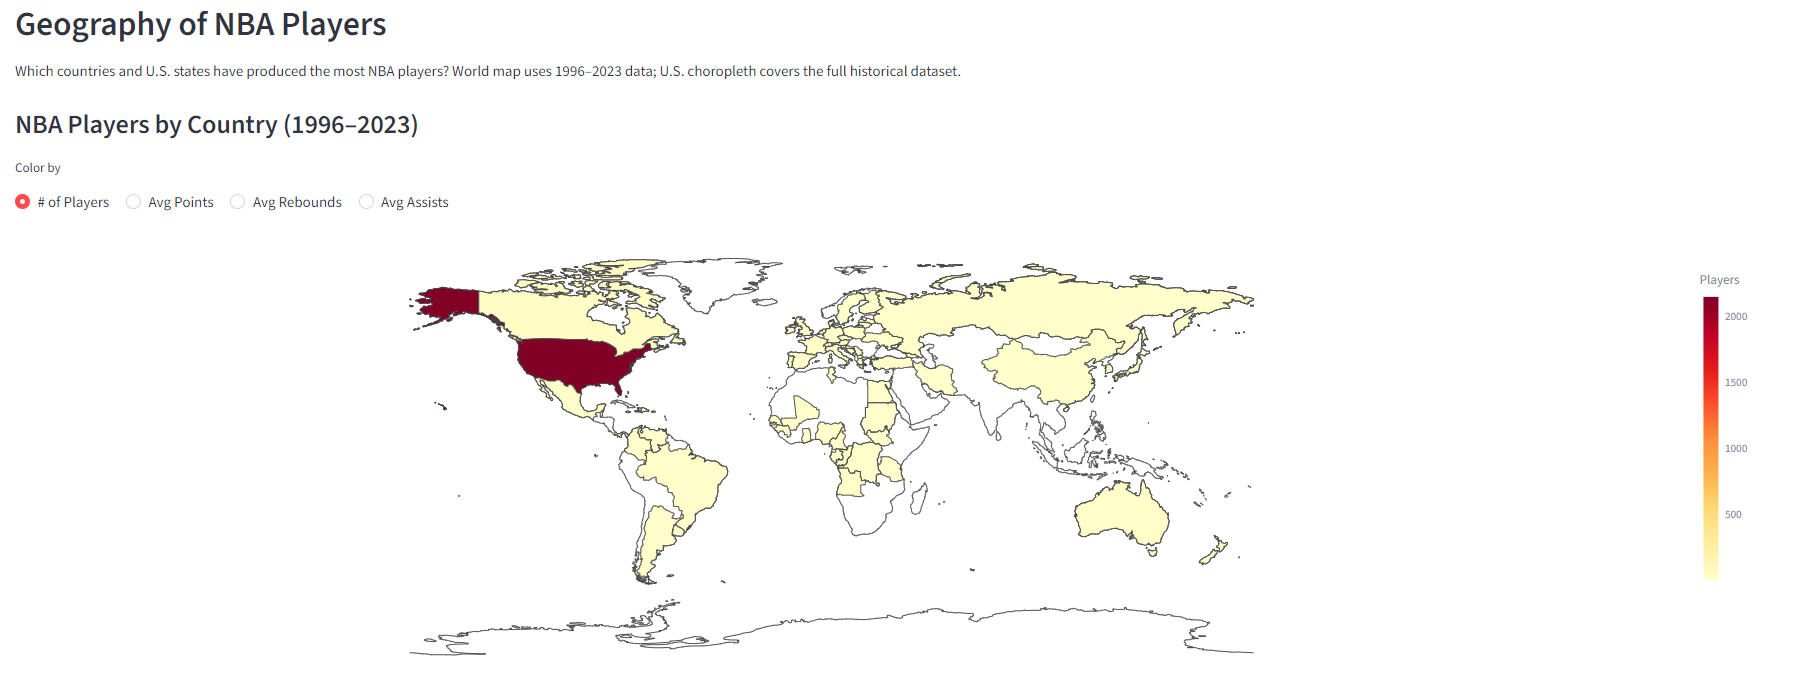
\includegraphics[width=\columnwidth]{figures/report/fig4.png}
  \caption{World choropleth of NBA player origins (1996--2023). USA: 10,721 player-seasons; top non-US: Canada (205), France (190), Australia (100), Spain (93).}
  \label{fig:world}
\end{figure}

\begin{figure}[H]
  \centering
  % ── HOW TO GET THIS FIGURE ──────────────────────────────────────────────
  % Still in Tab 4 -- scroll down past the bar chart
  % Take a screenshot of the U.S. state choropleth
  % Save as fig5.png
  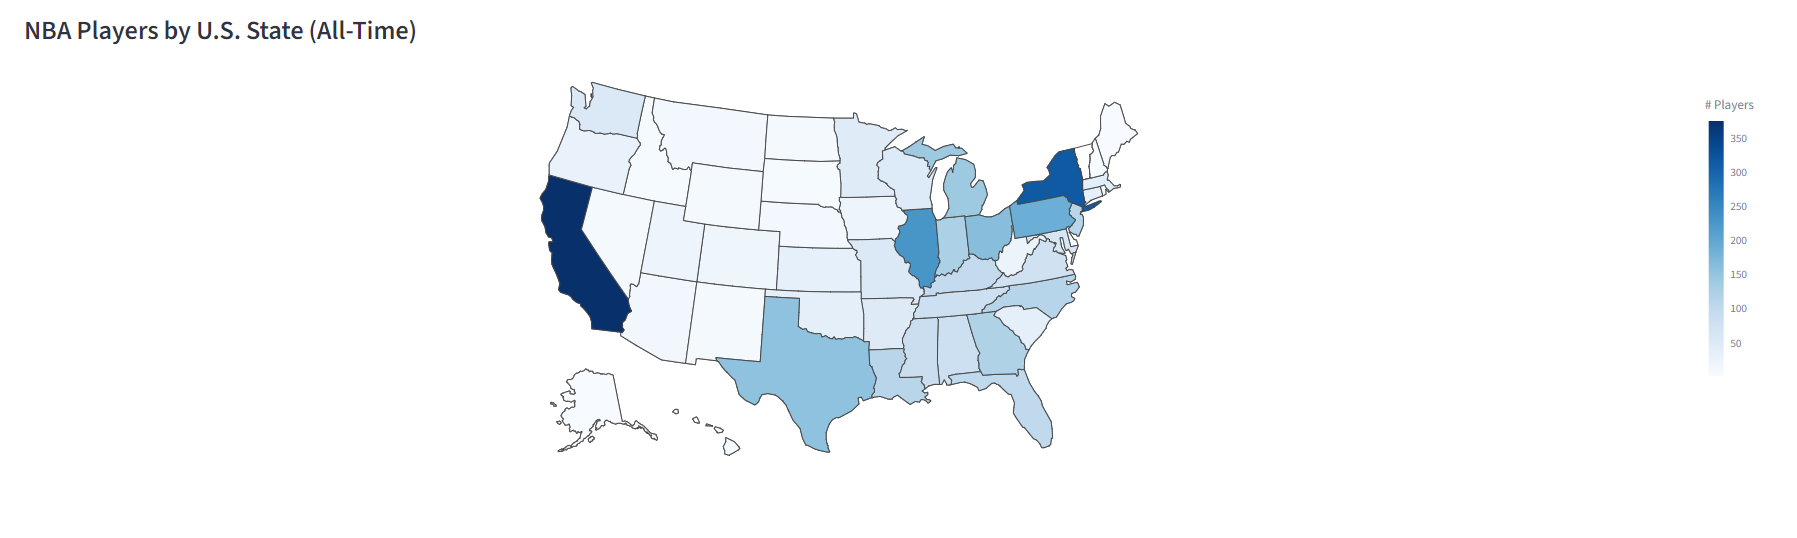
\includegraphics[width=\columnwidth]{figures/report/fig5.png}
  \caption{All-time NBA player count by U.S. birth state. California, New York, and Texas are the top producing states.}
  \label{fig:states}
\end{figure}

\subsection{RQ5 -- Position Profiles}

Per-game and advanced statistics (1947--2024, min.\ 20 games/season) are combined and grouped by primary position (PG, SG, SF, PF, C). A normalized position $\times$ statistics heatmap (11 metrics), a box plot for a user-selected metric, and a radar chart showing mean normalized profiles are provided.

\begin{figure}[H]
  \centering
  % ── HOW TO GET THIS FIGURE ──────────────────────────────────────────────
  % Navigate to Tab 5 "Position Profiles"
  % Select all 5 positions, Era: All
  % Take a screenshot showing the heatmap (top) and radar chart (bottom)
  % Save as fig6.png
  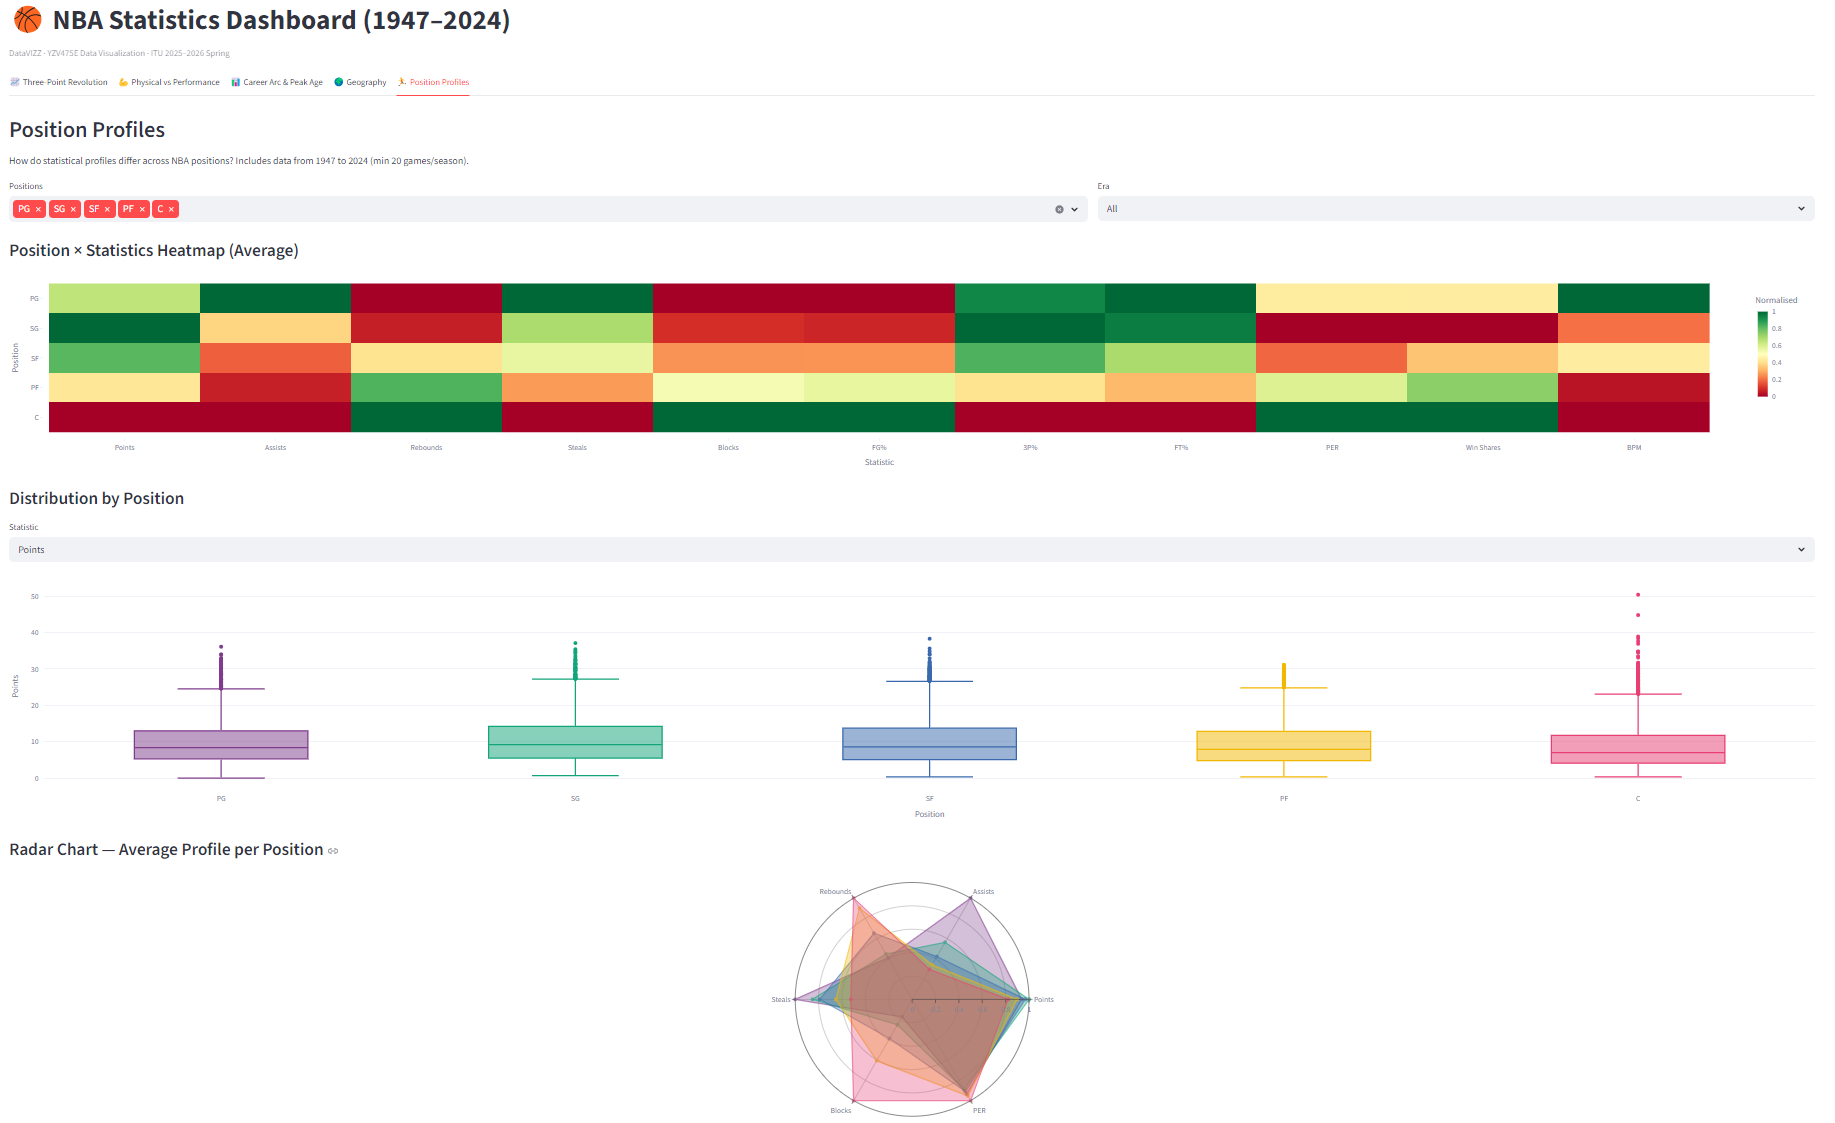
\includegraphics[width=\columnwidth]{figures/report/fig6.png}
  \caption{Position profiles: (top) normalized position $\times$ statistics heatmap; (bottom) radar chart of mean profile per position (PPG, APG, RPG, SPG, BPG, PER).}
  \label{fig:positions}
\end{figure}

Key finding: PGs lead in assists and 3P\%; centers dominate blocks, rebounds, and Win Shares; small forwards show the most balanced profiles. The era filter reveals that positional boundaries have blurred significantly in the modern period.

% ── IV. Implementation ────────────────────────────────────────────────────────
\section{Technical Implementation}

The dashboard is a multi-tab Streamlit~\cite{streamlit} application. Data loading is centralized in \texttt{data\_loader.py} with \texttt{@st.cache\_data} to avoid repeated 11~MB reads across tab switches. Each of the five tabs is implemented as an independent module (\texttt{tabs/tab\_*.py}). All charts use Plotly~\cite{plotly} for interactive hover, zoom, and filter support. OLS trendlines use \texttt{statsmodels}~\cite{statsmodels}. The full stack is Python~3.10, Pandas, and NumPy.

To run: \texttt{pip install -r requirements.txt} followed by \texttt{streamlit run app.py}.

% ── V. Conclusion ─────────────────────────────────────────────────────────────
\section{Conclusion}

The dashboard demonstrates that NBA statistics provide a rich, multi-dimensional dataset well-suited to interactive visualization. The five research questions collectively reveal: (1) a fundamental tactical shift driven by the three-point rule, (2) weak but interpretable relationships between physicality and performance, (3) a consistent career peak at age 26--27, (4) rapid globalization since 2000, and (5) distinct but converging positional roles. The Streamlit application enables exploratory analysis beyond static charts through dynamic filters for era, position, country, and metric.

% ── References ────────────────────────────────────────────────────────────────
\begin{thebibliography}{9}

\bibitem{main_dataset}
S. Rodatta, ``NBA Stats (1947--present),''
\textit{Kaggle}, 2024. [Online]. Available:
\url{https://www.kaggle.com/datasets/sumitrodatta/nba-aba-baa-stats}

\bibitem{justinas_dataset}
Justinas, ``NBA Players Data (1996--2023),''
\textit{Kaggle}, 2023. [Online]. Available:
\url{https://www.kaggle.com/datasets/justinas/nba-players-data}

\bibitem{birthplace_dataset}
thedevastator, ``Birthplaces of NBA and ABA Players,''
\textit{Kaggle}, 2023. [Online]. Available:
\url{https://www.kaggle.com/datasets/thedevastator/birthplaces-of-nba-and-aba-players}

\bibitem{streamlit}
Streamlit Inc., ``Streamlit Documentation,'' 2024. [Online]. Available:
\url{https://docs.streamlit.io}

\bibitem{plotly}
Plotly Technologies Inc., ``Plotly Python Open Source Graphing Library,''
2024. [Online]. Available: \url{https://plotly.com/python}

\bibitem{statsmodels}
S.~Seabold and J.~Perktold, ``statsmodels: Econometric and statistical
modeling with Python,'' in \textit{Proc. 9th Python in Science Conf.}, 2010.

\end{thebibliography}

\end{document}
